\documentclass{estilo}
\usepackage[spanish]{babel}
\usepackage{graphicx}
\usepackage{float}
\usepackage{amsmath}        % para los vectores columnas
\usepackage{amsfonts}       % para las negrita de pizarra
\usepackage{amssymb}        % para simbolos matematicos
\usepackage{hyperref}       % para utilizar referencias
\usepackage{multirow}       % para las tablas
\usepackage{dsfont}
\usepackage{listings}
\usepackage{xcolor}
\definecolor{codegreen}{rgb}{0,0.6,0}
\definecolor{codegray}{rgb}{0.5,0.5,0.5}
\definecolor{codepurple}{rgb}{0.58,0,0.82}
\definecolor{backcolour}{rgb}{0.95,0.95,0.92}
\lstdefinestyle{mystyle}{
    backgroundcolor=\color{backcolour},   
    commentstyle=\color{codegreen},
    keywordstyle=\color{magenta},
    numberstyle=\tiny\color{codegray},
    stringstyle=\color{codepurple},
    basicstyle=\ttfamily\footnotesize,
    breakatwhitespace=false,         
    breaklines=true,                 
    captionpos=b,                    
    keepspaces=true,                 
    numbers=left,                    
    numbersep=5pt,                  
    showspaces=false,                
    showstringspaces=false,
    showtabs=false,                  
    tabsize=2
}
\lstset{style=mystyle}

\usepackage{enumitem,multicol,setspace}
\newcounter{subenum}[enumi] % para las multicolumnas
\renewcommand{\thesubenum}{\arabic{subenum}}
\usepackage[nomessages]{fp}
\FPeval\thecolwidth{round(1/4:4)}% Specify number of columns -> column width
\newcommand{\newitem}[1]{%
  \refstepcounter{subenum}%
  \parbox{\dimexpr\thecolwidth\linewidth-.5\columnsep}{%
    \makebox[\labelwidth][r]{(\thesubenum)\hspace*{\labelsep}}%
    #1}\hfill%
}

\usepackage{scalerel,stackengine} % para el sombrero
\stackMath
\newcommand\rhat[1]{%
\savestack{\tmpbox}{\stretchto{%
  \scaleto{%
    \scalerel*[\widthof{\ensuremath{#1}}]{\kern-.6pt\bigwedge\kern-.6pt}%
    {\rule[-\textheight/2]{1ex}{\textheight}}%WIDTH-LIMITED BIG WEDGE
  }{\textheight}% 
}{0.5ex}}%
\stackon[1pt]{#1}{\tmpbox}%
}
\parskip 1ex

\usepackage{mathtools}      % floor y ceil
\DeclarePairedDelimiter\ceil{\lceil}{\rceil}
\DeclarePairedDelimiter\floor{\lfloor}{\rfloor} 

\usepackage[style=authoryear-comp]{biblatex}

\begin{document}
\maketitle
\newpage
\section{Problema a solucionar}
\renewcommand{\labelenumii}{\arabic{enumi}.\arabic{enumii}}
\renewcommand{\labelenumiii}{\arabic{enumi}.\arabic{enumii}.\arabic{enumiii}}
\renewcommand{\labelenumiv}{\arabic{enumi}.\arabic{enumii}.\arabic{enumiii}.\arabic{enumiv}}

Luego de haber analizado a todos los rivales gracias a tu ayuda, Scaloni definió
un cronograma de entrenamiento. Tiene definido qué hacer para cada día de acá
al mundial que viene, e incluso más. Para hacerlo más simple, para los próximos $n$
días. El entrenamiento del día $i$ demanda una 
cantidad de esfuerzo $e_i$, y podemos decir que la ganancia que nos da
dicho entrenamiento es igual al esfuerzo. El entrenamiento 
que corresponde al día $i$ (así como su esfuerzo y ganancia) son inamovibles: 
el Chiqui Tapia alquiló las herramientas específicas para cada día, y la AFA 
está muy ocupada organizando el torneo de $2^{30}$ equipos del año que viene para 
andar moviendo cosas. Si la cantidad de energía que se tiene para un día $i$
es $j < e_i$, entonces la ganancia que se obtiene en ese caso es justamente $j$.
(si se tiene más energía que $e_i$, no es que se pueda usar más para tener más ganancia).

A su vez, los jugadores no son máquinas. La cantidad de energía que tienen disponible
para cada día va disminuyendo a medida que pasan los entrenamientos. Suponiendo
que los entrenamientos empiezan con los jugadores descansados, el primer
día luego de dicho descanso los jugadores tienen energía $s_1$. El segundo día
luego del descanso tienen energía $s_2$, etc... Para cada día
hay una cantidad de energía, y podemos decir que $s_1 \geq s_2 \geq ... \geq s_n$.
Scaloni puede decidir dejarlos descansar un día, haciendo que la energía "se renueve"
(es decir, el próximo entrenamiento lo harían con energía $s_1$ nuevamente,
siguiendo con $s_2$, etc...). Obviamente, si descansan, el entrenamiento de ese
día no se hace (y no se consigue ninguna ganancia).   

Scaloni no sabe bien cómo hacer para definir los días que deba entrenarse y los días
que convenga descansar de tal forma de tener la mayor ganancia posible (y tener
mayores probabilidades de ganar el mundial que viene), pero Menotti, 
exponente del juego bonito en Argentina, le recomendó usar Programación Dinámica
para resolver este problema. Nos está pidiendo ayuda para poder resolver este
problema. 

\subsection{Nota }

        Esta versión del informe contiene las correcciones solicitadas, los segmentos con titulos que contengan un "*" contienen correcciones 
        
\subsection{Algunas reglas a considerar}

\begin{enumerate}
    \item Se poseen dos conjuntos $E_i \text{ y } S_j$ donde corresponden al esfuerzo a realizar en un dia i y la energia disponible para un dia j, respectivamente
\item $\lvert E_i \lvert \ = \lvert S_j \lvert$ 
\item Se construye una función esfuerzo cuya representación matematica seria:
$
Esfuerzo(E_i, S_j) = \begin{cases}
  E_i & \text{si }  E_i < S_j\\
  S_j & \text{si }  E_i > S_j\\
  0 & \text{si }  j <= 0 \text{ o }  i <=0 \\
\end{cases}
$
\item Del enunciado sabemos que $S_{k+1} \le S_k$
\item Para un esfuerzo $E_i$ solo se podra agregar a la solucion si se incluye antes de un dia $S_j$ con $i \leq j$ 
\end{enumerate}
\section{Construyendo la ecuación de recurrencia *}

Analicemos como se comporta el problema en un principio, la solución trivial de este problema seria basicamente pensar que si no debo entrenar entonces mi ganancia es 0 y esto se puede expresar como:

- El optimo de $E_0$ (que en otras palabras es $\empty$) es 0 , asumiendo también que la energia que se tiene disponible es $S_0 = \empty$, expresado en terminos de una ecuación de recurrencia esto seria $T(E_0, S_0) = 0$

Ahora teniendo tan solo un entrenamiento se debe considerar claramente tambien la energia para ese día de entrenamiento: 

- Esto lo podemos resumir en terminos de la función esfuerzo como $T(E_1, S_1) = esfuerzo(E_1, S_1)$

Ahora si se tienen dos días se puede decir algo similar a lo anterior, pero en este caso vale observar algunas cosas que son intesantes, en este caso se tienen tan solo dos posibilidades:

- La primera es que se entrena solo el segundo dìa porque la ganancia es superior a la suma de entrenar ambos dias $T(E_2, S_1) = esfuerzo(E_2, S_1)$
- La segunda es se entrenan ambos dias, lo cual en terminos de la función esfuerzo es: $T(E_2, S_2) = esfuerzo(E_2, S_2) + esfuerzo(E_1, S_1)$

Es importante observar que teniendo dos elementos nunca va a ser conveniente dejar de entrenar el ultimo día, puesto que no importa que tan grande sea el esfuerzo del primer día siempre con la energía restante conviene hacer un entrenamiento pues este sumara alguna ganancia más (a menos que la energia restante sea 0)

Por otro lado, que pasa si debo considerar 3 días, se puede observar que es necesario obtener el maximo entre estas 3 posibilidades:
 

$$
\begin{align*}
&\text{Entreno el primer y tercer día: } esfuerzo(E_3, S_1) + esfuerzo(E_1, S_1) \\
&\text{Entreno el segundo día y el tercero: } esfuerzo(E_3, S_2) + esfuerzo(E_2, S_1) \\
&\text{Entreno los 3 días: } esfuerzo(E_3, S_3) + esfuerzo(E_2, S_2) + esfuerzo(E_1, S_1) \\
\end{align*}
$$

En el caso de tener 4 dias de entrenamiendo se debe considerar los mismos casos que ocurren en el analisis de tener 3 elementos, pero esta vez se agregan a todos el entrenamiento del cuarto dia con la energia correspondiente, segun lo determina la funcion de esfuerzo, a su vez, también añadir la posibilidad de no entrenar el tercer dia y entrenar tan solo el segundo y cuarto dia con las energias renovadas, entonces se consiguen las siguientes posibilidades para el entrenamiento:

$$
\begin{align*}
&\text{Entreno el primero, el tercero y el cuarto } \rightarrow esfuerzo(E_1, S_1) + esfuerzo(E_3, S_1) + esfuerzo(E_4, S_2)\\
&\text{Entreno el segundo, el tercero y el cuarto } \rightarrow esfuerzo(E_2, S_1) + esfuerzo(E_3, S_2) + esfuerzo(E_4, S_3)\\
&\text{Entreno los 4 días de corrido } \rightarrow esfuerzo(E_1, S_1) + esfuerzo(E_2, S_2) + esfuerzo(E_3, S_3) + esfuerzo(E_4, S_4)\\
&\text{Entreno el primero, el segundo y el cuarto } \rightarrow esfuerzo(E_1, S_1) + esfuerzo(E_2, S_2) + esfuerzo(E_4, S_1)\\
&\text{Entreno el segundo y el cuarto } \rightarrow esfuerzo(E_2, S_1)+ esfuerzo(E_4, S_1)\\
\end{align*}
$$

Observar que en el ejemplo anterior se construyen las respuestas agregando la extensión correspondiente al cuarto día y la cuarta posibilidad corresponde a la que se agrega por la extensión del tamaño de la entrada

De esta manera y viendo como se van construyendo las respuestas, se puede construir una generalización mediante una ecuación de recurrencia que abarque todas las posibilidades, dicha ecuación viene dada de la siguiente manera:

$$
\\
T(E_i, S_j) = max\begin{cases}
  T(E_{i-2}, S_{j-2}) + esfuerzo(E_{i}, S_1) \\
  T(E_{i-1}, S_{j-1}) + esfuerzo(E_i,S_j) \\
  T(E_i, S_{j-1})                                          
\end{cases} 
\\
$$

Esto claro, considerando los casos base:

$$
T(E_1, S_1) = esfuerzo(E_1, S_1) \\
T(E_2, S_1) = esfuerzo(E_2, S_1) \\ 
T(E_2, S_2) = esfuerzo(E_2, S_2) + esfuerzo(E_1, S_1)\\
\text{si } i \ o \ j \le 0 \rightarrow T(E_i, S_j) = 0
$$
\section{Codigo solución *}

En un principio se agrega la implementación de la función esfuerzo la cual es vital para poder solucionar el problema mediante la tecnica de programación dínamica:


\begin{lstlisting}[language=Python]
def funcion_esfuerzo(i: int, j: int, esfuerzo: list, energia: list):
    return energia[j] if esfuerzo[i] > energia[j] else esfuerzo[i]
\end{lstlisting}

Una vez habiendo construido la ecuación de recurrencia se puede construir el codigo solución del problema utilizando la tecnica button-up para evitar llamados de recurrencias inecesarios que realenticen el problema

\begin{lstlisting}[language=Python]
def explorar_espacion_solucion(esfuerzo: list, energia: list):
    n = len(esfuerzo)
    espacio_solucion = [[0 for _ in range(n)] for _ in range(n)]

    espacio_solucion[0][0] = funcion_esfuerzo(0, 0, esfuerzo, energia)
    espacio_solucion[1][0] = funcion_esfuerzo(1,0, esfuerzo, energia)
    espacio_solucion[1][1] = max(funcion_esfuerzo(1,1, esfuerzo, energia) + espacio_solucion[0][0], espacio_solucion[1][0])

    for i in range(2, n):
        for j in range(i + 1):
            if j == 0:
                espacio_solucion[i][0] = espacio_solucion[i-2][i-2] + funcion_esfuerzo(i, 0, esfuerzo, energia)
            else:
                espacio_solucion[i][j] = max([espacio_solucion[i-1][j-1] + funcion_esfuerzo(i, j, esfuerzo, energia), espacio_solucion[i][j-1], espacio_solucion[i-2][j-2] + funcion_esfuerzo(i,0, esfuerzo, energia)])
    return espacio_solucion, espacio_solucion[n-1][n-1]
\end{lstlisting}

El codigo anteriormente dado contiene la solución por programación dínamica y haciendo uso de la memoización del metodo, se aprovecha tambien retornar la matriz con la exploración de las posibles respuestas de manera que sea posible realizar una reconstrucción en la secuencia de entrenamiento para poder saber que hacer cada día

Por otro lado, se agrega el codigo solución de la reconstrucción de la secuencia de entrenamiento, el cual será explicado en la siguiente sección del informe

\begin{lstlisting}[language=Python]
def _encontrar_secuencia(espacio_solucion: list, secuencia: str, n: int):
    if n < 0:
        return
    if n == 0 and len(secuencia) < len(espacio_solucion):
        secuencia.append("Entreno")
        return
    indice = espacio_solucion[n].index(max(espacio_solucion[n]))
    indice += 1
    for _ in range(indice):
        secuencia.append("Entreno")
    if len(secuencia) < len(espacio_solucion):
        secuencia.append("Descanso")
    n -= indice + 1
    return _encontrar_secuencia(espacio_solucion, secuencia, n)
 
def encontrar_secuencia_entrenamiento(espacio_solucion: list):
    secuencia = []
    _encontrar_secuencia(espacio_solucion, secuencia, len(espacio_solucion) - 1)
    secuencia.reverse()
    return secuencia
\end{lstlisting}
\input{tex/4_Reconstrucción de la secuencia de entrenamiento}
\section{Analizando la complejidad temporal}

\subsection{Obtención del maximo}
Dada la observación al inicio del informe se sabe que las listas de entrada de esfuerzo y energia cumplen con $\lvert E_i \lvert \ = \lvert S_j \lvert$ por lo tanto en un principio se tendría rapidamente y sin profundizar que:

$$
T(n) = O(n²) \text{ siendo n el tamaño de cualquiera de las dos entradas}
$$

En un principio observamos el comportamiento del algoritmo para algunos elementos y observamos la curva de medicion empìrica:

\begin{figure}[H]
    \centering
    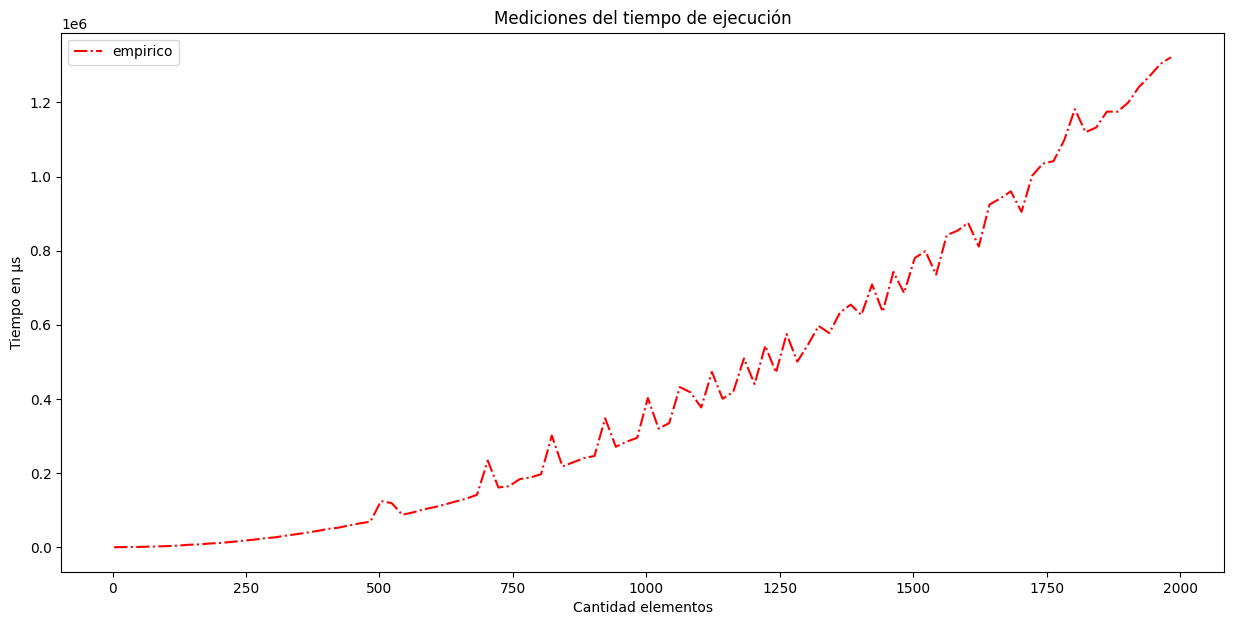
\includegraphics[width=1\textwidth]{graficos/tiemposejecucion.png}
\end{figure}

En la grafica anterior podemos observar la duración en microsegunos del tiempo de ejecución del algoritmo para un conjunto de datos aleatorios en el rango de cero y dos mil elemenos

Por otro lado, se realiza una curva teorica de la complejidad, del tipo cuadratica que resulta de elevar al cuadrado la longitud del cardinal de alguno de los dos conjuntos 

\begin{figure}[H]
    \centering
    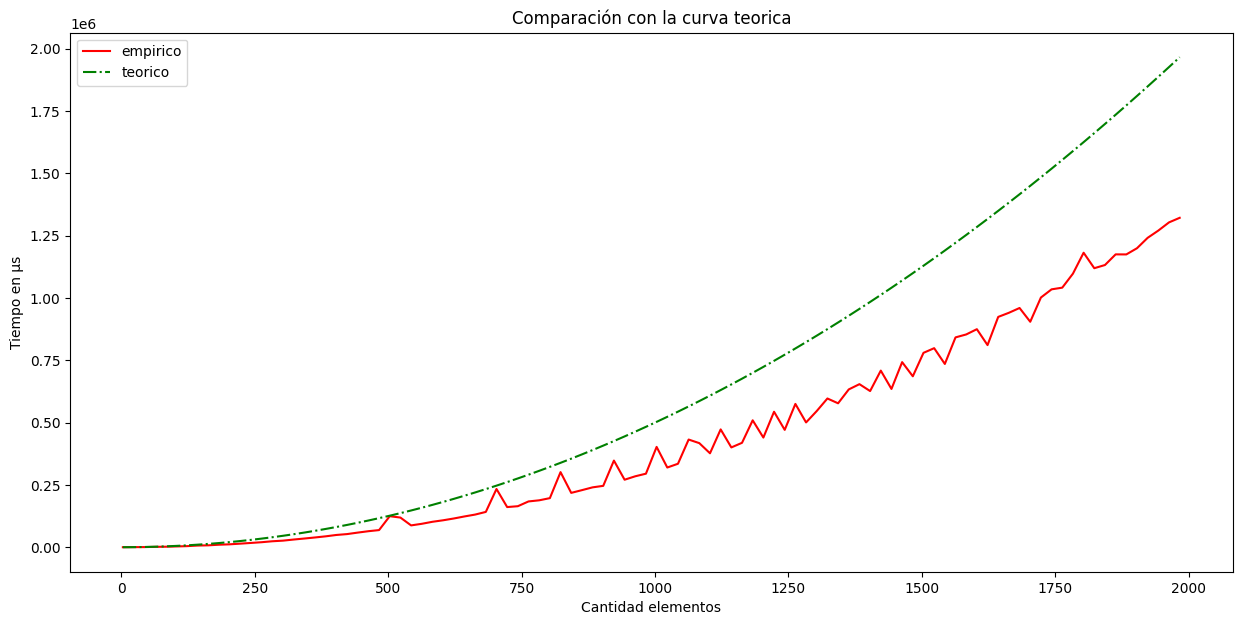
\includegraphics[width=1\textwidth]{graficos/vsteorica.png}
\end{figure}

La grafica contiene la medicion anteriormente realizada pero esta vez se compara tambien contra un tiempo teorico estimado, en un principio pareceria que el algoritmo se encuentra correctamente acotado por el tiempo teorico.

Ahora es importante analizar otros aspectos del problema, se debe verificar que este no tenga un comportamiento diferente respecto la longitud en bits de la entrada, en otras palabras, habra que verificar si este algoritmo cumple o no con ser de caracter pseudopolinomial

Analicemos primero como se comporta la longitud en bits del tamaño de la entrada, es importante ver que la longitud en bits del tamaño de la entrada va a ser constante en determinados rangos, y dando un ejemplo de esto, para 8 y 10 necesito la misma cantidad de bits para representarlos dentro del computador, esto es pues que necesito $\log_2(n)
$ digitos para representar el valor. Como en el dominio del problema siempre voy a tener que la longitud de la entrada es igual para cada conjunto, la variabilidad segun esta crece no es significativa para el problema y esto significa que para determinados rangos de los valores de entrada el generar la matriz del espacio de solución puede verse como una constante. 

Para validar dicha idea, hace falta realizar una grafica en escala logaritmica (por un tema de comodidad) en donde se grafica la longitud en bits de la entrada en contra del logaritmo de la medición realizada anteriormente, en caso de encontrar que estos datos se comportan de manera lineal en la escala, se habra determinado empiricamente que dicho algoritmo es de caracter pseudopolinomial. Y por lo tanto seria una prueba para eliminar la cota teorica anteriormente planteada

\begin{figure}[H]
    \centering
    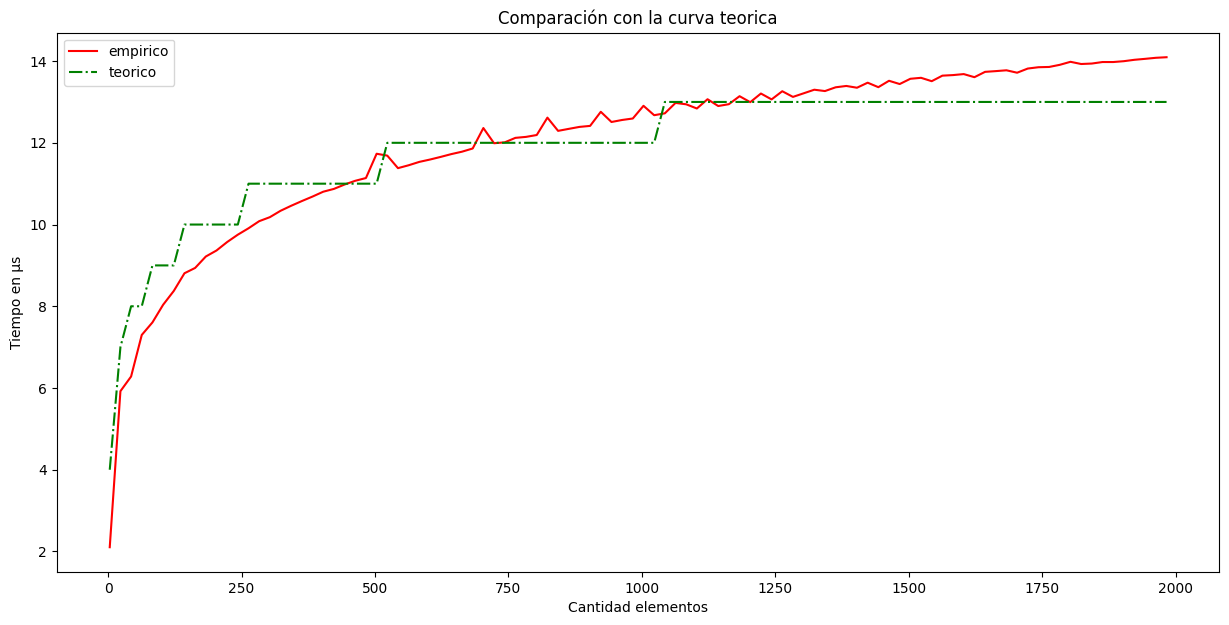
\includegraphics[width=1\textwidth]{graficos/logaritmica.png}
\end{figure}

La grafica anterior, sirve como un metodo empirico para refutar un supuesto comportamiento pseudopolinomial del algoritmo. Por lo tanto la cota temporal en notación Big O obtenida en un principio sigue sostenida por las pruebas de medición realizadas en el analisis. Finalmente se afirma con mayor criterio que:

$$
 T(n) = O(n²)
$$

Donde L es la longitud de la entrada del esfuerzo o la energia 

\subsection{Reconstrucción de secuencia}
Reconstruir la secuencia depende de dos cosas: 

- Encontrar la posicion de un maximo en un arreglo
- Iterar k + 1 veces cada vez que la recurción llega a una fila nueva 

En este caso, se genero una funcion que hace  $T(n) = O(n)$, por otro lado, iterar k + 1 veces tambien cumple con ser lineal $T(n) = O(n)$.

En un principio dicho algoritmo para un caso generico parece ser también cumplir con ser $T(n) = O(n)$

Hay un gran pero en la complejidad anteriormente asignada, existe la posibilidad de que la secuencia de entrenamiento llegue a ser una secuencia alternada $(Entrenamiendo, Descanso, Entrenamiendo, ...)$, entonces se sabe que este algoritmo buscara la posicion del maximo un aproximado de $n/2$ lo cual es hacer algo lineal $n/2$ veces que se aproxima más a un caso cuadratico (se descartan las iteraciones realizadas en la reconstrucción de la secuencia porque son siempre de longitud 1), ahora como es muy particular podemos definir un comportamiento general y un peor caso. 

Entonces este algoritmo se comportaria de la siguiente manera:

$$
T(n) = O(n) \text{ para casos generales} \\
$$
T(n) = O(n^2) \text{ para el caso de tener una secuencia que sea siempre alternada} \\
$$
 \text{ siendo n la longitud de cualquier fila del espacio de solución}
$$

Se agrega una grafica con las mediciones temporales del algoritmo para comprobar su comportamiento estimado

\begin{figure}[H]
    \centering
    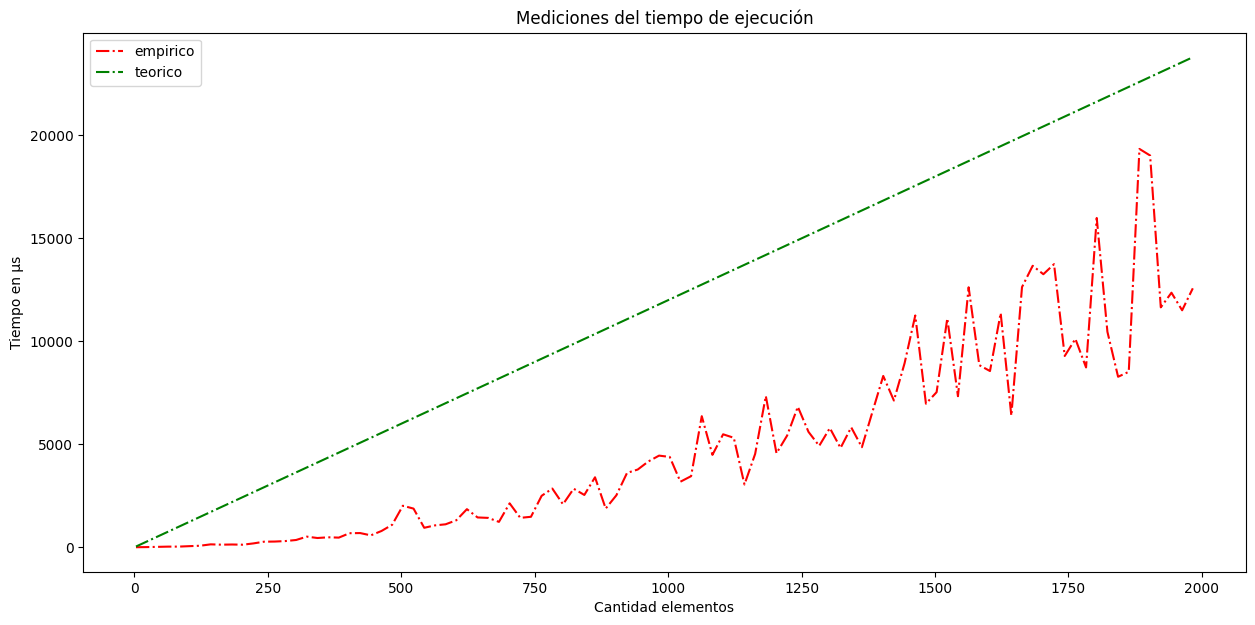
\includegraphics[width=1\textwidth]{graficos/reconstruccion.png}
\end{figure}

En esta grafica se puede comprobar que el comportamiendo del algoritmo tiene una tendencia de creciento lineal, tal como se estimaba, asi como tambien que la velocidad varia bastante dependiendo de la cantidad de saltos "descansos" que tenga la secuencia de entrenamiento. 
\section{Conclusiones}

En conclusión, este informe abordó el problema de planificar el entrenamiento de la selección de fútbol de Argentina de manera óptima, maximizando la ganancia total a lo largo de un período de tiempo dado. Se formuló una función de recurrencia que describe la mejor manera de tomar decisiones sobre cuándo entrenar y cuándo descansar, considerando el esfuerzo requerido y la energía disponible para cada día. 

Se demostró que la complejidad temporal del algoritmo propuesto es cuadrática en función de la longitud de las entradas de esfuerzo y energía, lo que significa que su tiempo de ejecución se encuentra acotado por una función polinómica. Esto es una buena noticia, ya que indica que el algoritmo es eficiente y escalable en la práctica.

Además, se realizaron mediciones empíricas que respaldaron la complejidad teórica, mostrando que el tiempo de ejecución del algoritmo se comporta de manera consistente con una complejidad cuadrática en la longitud de las entradas. No se encontraron indicios de un comportamiento pseudopolinomial, lo que refuerza la validez de la cota temporal.

En resumen, este informe proporciona una solución eficiente y escalable para el problema de planificar el entrenamiento de la selección de fútbol de Argentina, respaldada por análisis teóricos y mediciones empíricas. Esto debería permitir que el equipo técnico tome decisiones informadas sobre cómo estructurar el entrenamiento para maximizar las posibilidades de éxito en el próximo Mundial.
\end{document}